\subsection{Systematic/Property Name}

\paragraph{Description:}
For a constant position of the HWP, the polarization angle of the HWP is the 
direction along which an input polarized signal results in a maximum (or minimum) output signal
from the HWP. Any error in the measurement of this angle results in absolute angle calibration error. The HWP polarization angle depends 
on both the frequency (see Sec.) and the incidence angle of the incoming radiation.


\paragraph{Plan to model and/or measure:}
To probe the polarization angle dependance versus the incidence angle Fourier Transform Spectrometer measurements with a constant 
input polarized signal versus the HWP at different incident angles can be performed.

\paragraph{Uncertainty/Range:}
The detector angles, the polarization angle of the input signal, and the
HWP angle should be known reasonably well.


\paragraph{Parameterization:}
The parametrization, and simulation, of the HWP polarization angle is pretty simple once the ordinary and extraordinary refraction indices
of a birifringent material, or their equivalents for a metamaterial HWP, are known/measured versus frequency/incident angle.


\begin{figure}
\centering
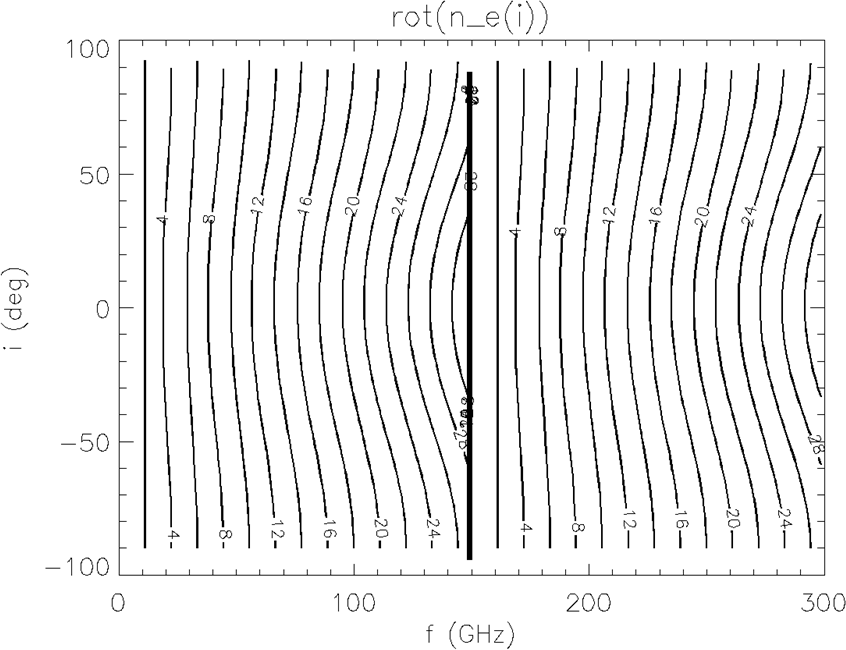
\includegraphics[width=2.5in]{figures/polanglei.png}
\caption{Sapphire HWP polarization angle versus frequency and incidence angle. The plot shows the rotation angle in degrees.}
\label{4pixelwobbleremoval}
\end{figure}
